\documentclass[a4 paper,12pt]{article}
\usepackage[margin=1.3cm]{geometry}
\usepackage{graphicx}
\title{\bfseries\Huge Omkar Mohite}
\author{Student, \textbf{T.Y.B.Tech EXTC, VJTI}, Matunga, Mumbai.\\\textbf{Mobile No.:} +91 9820774749\\\textbf{email-id:} mohiteomkar46@gmail.com\\\textbf{Residential Address:} 96/503, B-wing, Shubh CHS,\\ Tilak nagar, Chembur, Mumbai-400089.\\}
\date{}

\begin{document}
	\begin{minipage}{0.75\textwidth}
		\begingroup
		\let\endcenter\endflushleft
		\maketitle
		\endgroup
	\end{minipage}
	\begin{minipage}{0.2\textwidth}
		\graphicspath{ {images/} }
		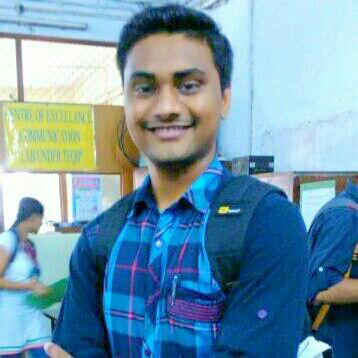
\includegraphics[width=4cm, height=4cm]{IMG-20140509-WA0002}
	\end{minipage}


\begin{minipage}{0.98\textwidth}
	\section{Career Objective:}
	\vspace{-0.1in}
	To seek an opportunity in which I can showcase my talent in problem solving environment so that it turns an asset for the organization and to work in boosting and challenging environment.\\\\
\end{minipage}

\begin{minipage}{0.98\textwidth}
\section{Education:}
\vspace{-0.1in}
\begin{center}
	\begin{tabular}{|p{1.5cm}|p{2cm}|p{5cm}|p{4.5cm}|p{2.5cm}|}
		\hline
		\textbf{Sr.No.} & \textbf{Year} & \textbf{Examinations} & \textbf{Institute} & \textbf{Grades}\\ [0.5ex] 
		\hline
		1. & 2014-15 &3rd Year B.Tech. in EXTC & Veermata Jijabai Technological Institue, Mumbai-400019. & 8.6 CPI \\ 
		\hline
		2. & 2013 & Diploma in Industrial Electronics Engineering & K. J. Somaiya Polytechnic, Vidyavihar, Mumbai-400077.& 94.13 percent \\
		\hline
		3. & 2010 & S.S.C. & Lokmanya Tilak High School, Tilak Nagar, Chembur, Mumbai-400089. & 94.36 percent \\
		\hline
	\end{tabular}
\end{center}

\section{Projects:}
\begin{enumerate}
	\vspace{-0.1in}
	\item\textbf{Automatic Irrigation Control System (Final year Diploma):}\\
	The aim of the project was to reduce the waste of water and human work required while drawing water in the farms. In this project we made use of copper wire as a soil moisture sensor based on its resistivity property, so that it could detect the requirement of water in the field and automatically turn on/off the motors when required.
	\item\textbf{Bomb Disposal Robot using Wireless Technology (Second Year Engineering):}\\
	The idea of the project was to eliminate the human risk involve in disposing bomb. We used the RF Module and software skills involved were Visual Basic, AVR Programming.
\end{enumerate}

\section{Training and Internship:}
\begin{itemize}
	\vspace{-0.1in}
	\item No internship yet.\\\\
\end{itemize}
\end{minipage}

\begin{minipage}{0.98\textwidth}
	\section{Research Publications:}
	\begin{enumerate}
		\vspace{-0.1in}
		\item Review on 'An Efficient Digital Implementation of
		Multicarrier CDMA System Based on Generalized DFT Filter Banks.'
		\item Review on 'Extra Matters Recognition of Transmission System Based on Hough Transform.'
	\end{enumerate}
\end{minipage}

\begin{minipage}{0.98\textwidth}
	\section{Technical Skills:}
	\begin{itemize}
		\vspace{-0.1in}
		\item C/C++ Programming and Object Oriented Programming
		\item Basic Knowledge about Android Application Development using Eclipse
		\item Simulation tools including MATLAB, SCILAB
		\item HTML
		\item Computer Networking
	\end{itemize}

\section{Soft Skills:}
\begin{enumerate}
	\vspace{-0.1in}
	\item Good Communication skills
	\item Adaptive Nature
	\item Good Teamwork and collaboration quality
\end{enumerate}

\section{Extra Curricular Activities:}
\begin{itemize}
	\vspace{-0.1in}
	\item Won eYantra, IIT-Bombay Robotics competition 2014-2015 in cargo sorting theme. (team of 4 members)
	\item Won State Level Technical Quiz Competition in Diploma held in the year 2012-13.(team of 3 members)
	\item Made a 'Restaurant Finder' android application in Credit Suisse Coding challenge for internship in year 2013-14.(team of 2 members)
	\item Participated in State level Technical Quiz Competition held at Shri Bhagubhai Mafatlal Polytechnic in the year 2012-13.
\end{itemize}

\section{Co-curricular Activities:}
\begin{enumerate}
	\vspace{-0.1in}
	\item Ranked 4th in Maharashtra in Diploma in Electronics Engineering and 9th in Maharshtra in all Diploma branches in the year 2013.
	\item Ranked 2nd in school in std 10th in SSC board.
\end{enumerate}
\end{minipage}

\end{document}